\documentclass[11pt]{article}

\setlength{\oddsidemargin}{-0.25 in}
\setlength{\evensidemargin}{-0.25 in}
\setlength{\topmargin}{-0.9 in}
\setlength{\textwidth}{7.0 in}
\setlength{\textheight}{9.0 in}
\setlength{\headsep}{0.75 in}
\setlength{\parindent}{0.3 in}
\setlength{\parskip}{0.1 in}
\usepackage{epsf}
\usepackage{pseudocode}
\usepackage{enumitem}
\usepackage{amsmath}
\usepackage{amssymb}
\usepackage{color}
\usepackage[normalem]{ulem}
\usepackage{graphicx}
\usepackage[export]{adjustbox}
\pagenumbering{arabic}
\def\O{\mathop{\smash{O}}\nolimits}
\def\o{\mathop{\smash{o}}\nolimits}
\newcommand{\e}{{\rm e}}
\newcommand{\R}{{\bf R}}
\newcommand{\Z}{{\bf Z}}

%% display solutions or not
\newif\ifsol
\soltrue % comment out to hide solutions

%% todo tracker -- overleaf v2 has better one it uses but will default to this if compiled on something that doesn't have built-in todo
\newcommand{\todo}[1]{\textbf{\textcolor{red}{#1}}}

\title{Section 4: MDPs}
\author{CS 182 - Artificial Intelligence}
\date{}
\begin{document}
\maketitle


\renewcommand{\labelenumii}{\arabic{enumii}.}
\setlength{\parindent}{0pt}

Recall that a \textbf{Markov Decision Process} is defined by
\begin{itemize}
  \item $S$: the set of possible \underline{states}

  \item $A$: the set of possible \underline{actions}, which may vary
  from state to state

  \item $T(s, a, s') \rightarrow \mathbb{R}$:
  the \underline{transition function} is the probability
  that $a$ from $s$ leads to $s'$

  \item $R(s, a, s') \rightarrow \mathbb{R}$:
  the \underline{reward function}. This could also be
  listed as $R(s')$ or $R(s,a)$

  \item The \underline{starting state}

  \item And, potentially, a \underline{terminal state}
\end{itemize}

With MDPs, we want to find the optimal policy $\pi^*: S \rightarrow A$,
which maximizes the expected utility.

Since we need to maximize the expected utility, we need that utility to be finite. We can acomplish this in one of three ways:

\begin{enumerate}
  \item \underline{Choosing a finite horizon}: By terminating the game after $T$ steps the reward must be finite. This often generates nonstationary policies, as $\pi$ depends on time remaining.
  
  \item \underline{Discounting over an infinite horizon}: Multiplying rewards by the discount rate $0 < \gamma < 1$ every time a new step is made will cause the solution to converge to a finite return and thus a finite solution, where a smaller discount rate ($\gamma$) leads to a shorter term focus.
  $$U([r_0, \cdots, r_\infty]=\sum_{t=0}^\infty \gamma^tr_t$$

  \item \underline{Have an absorbing state}: This will guarantee that for every policy a terminal state will eventually be reached.
\end{enumerate}

We define a \textbf{Q-state} $Q(s, a)$ as the expected utility of having taken action $a$ from state $s$ and acting optimally afterward:
$$Q^*(s,a) = \sum_{s'}T(s, a, s')[R(s, a, s') + \gamma V^*(s')]$$

And the \textbf{Value} of a state $V(s)$ as the expected utility of starting in $s$ and acting optimally. This can also be thought of as taking the best action $a$ at Q-state $Q(s,a)$:
$$V^*(s) = \max_a \sum_{s'}T(s, a, s')[R(s, a, s') + \gamma V^*(s')] = \max_a Q^*(s, a)$$

\textbf{Value Iteration} is a way to compute the optimal value for every state. It is done by first initializing the values for each state to 0:
$$V_0(S) = 0$$
Then the $k+1$ iteration will take the vector of $V_k(s)$ for all states $s$ and make a one step (Bellman) update:
$$V_{k+1}(s) = \max_a \sum_{s'} T(s, a, s') [R(s,a,s') + \gamma V_k(s')]$$

Unfortunately, this process is quite slow, as while the optimal action at each state (and thus the optimal policy) rarely changes, the optimal values can take many iterations to finally converge. Furthermore, each iteration is $O(S^2A)$ and thus the dimensionality and time complexity of the problem grows quite quickly with the size of the state or action space.

\textbf{Policy Iteration} attempts to overcome these issues by iteratively alternating between \textbf{Policy Evaluation} (updating the values) and \textbf{Policy Improvement} (updating the policy). This both reduces time complexity of the algorithm and allows it to exit earlier once the policy converges.

\textbf{Step 1: Policy Evaluation:} Starting with $V_k^{\pi_k}(s')$ and iterating (over $i$), update the values under a fixed policy $\pi_k$ until convergence:
$$V^{\pi_k}_{i+1}(s) = \sum_{s'} T(s, \pi_k(s), s') [R(s,\pi_k(s),s') + \gamma V_i^{\pi_k}(s')]$$
Call the converged values $V^{\pi_k}_{k+1}(s)$, and use them to update the policy:

\textbf{Step 2: Policy Improvement:} Extract a better policy based on these new values:
$$\pi_{k+1}(s) = \text{arg max}_a \sum_{s'} T(s, a, s') [R(s,a,s')+ \gamma V^{\pi_k}_{k+1}(s')] = \text{arg max}_a Q_{k+1}(s,a)$$

Note that Policy Evaluation is $O(S^2)$ operation and that both steps of Policy Iteration are easier to extract from the Q-values than the Values themselves.

\section*{Exercises}

\begin{enumerate}

\item For the environment shown below, calculate which squares can be reached from $(1,1)$ by the action sequence $[Up,Up,Right,Right]$ and with what probabilities. In this transition model, the probability of going in the intended direction is 0.8, but the agent travels in right angles to the intended direction with probability 0.1 each. A collision with a wall results in no movement.

\ifsol
  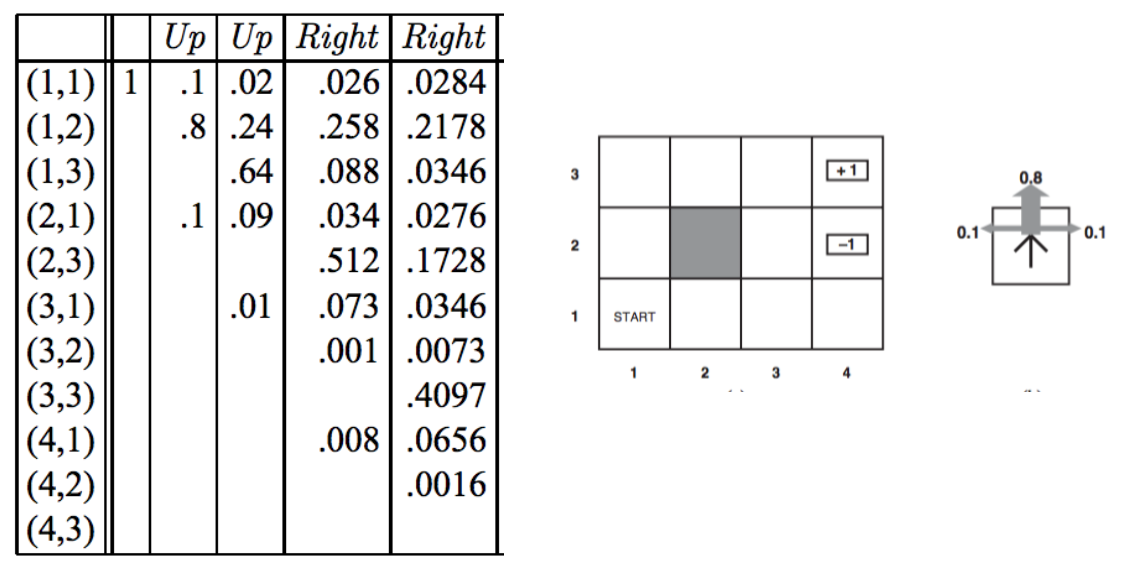
\includegraphics[scale=0.55, center]{img/actions_solution}
\else
  \bigskip
  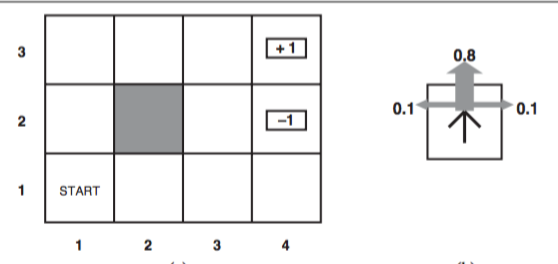
\includegraphics[scale=0.9, center]{img/environment}
\fi

\item Pacman is stuck in a friendlier maze where he gets a reward of $1$ every time he takes an action from state (0,0).  This setup is a bit
different from the one you have seen before:  Pacman can get the reward multiple times; these rewards do not get ``used up'' like food pellets and there are no ``living rewards.'' As usual, Pacman cannot move through walls and may take any of the following actions: go North ($\uparrow$), South ($\downarrow$), East ($\rightarrow$), West ($\leftarrow$), or stay in place ($\circ$).  State (0,0) gives a total reward of 1 every time Pacman takes an action in that state regardless of the outcome, and all other states give no reward. Actions are deterministic: each action will take Pacman in the correct direction unless Pacman runs into a wall, in which case he will remain in the same square.

\begin{enumerate}[label=\alph*)]
\item Assume a finite horizon of $h=10$ (so Pacman takes exactly 10 steps) and no discounting ($\gamma=1$).

\ifsol
  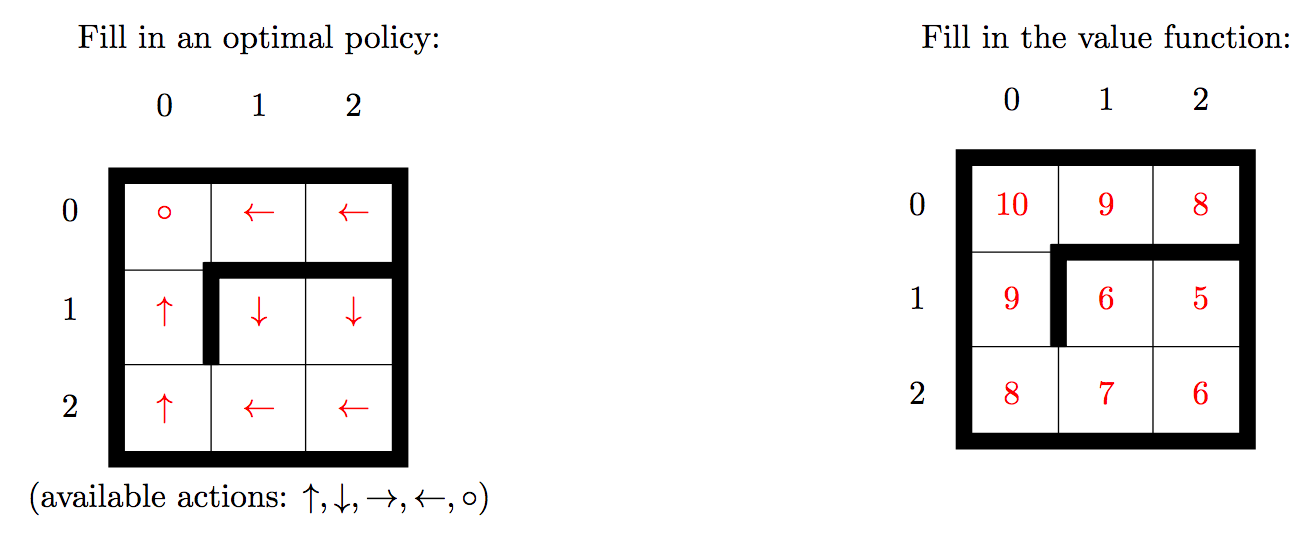
\includegraphics[scale=0.55, center]{img/maze_solutions}
\else
  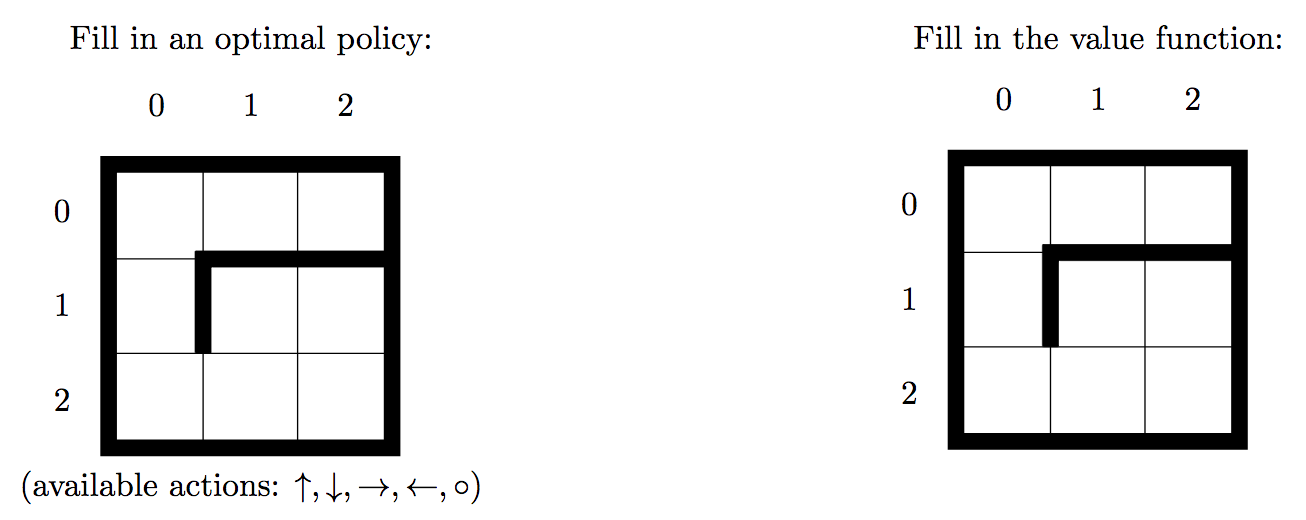
\includegraphics[scale=0.55, center]{img/maze}
\fi

\item Fill in following Q-values (with 10 steps remaining) corresponding to the value function you specified above.

The Q value of state-action (0,0), (East) is:

\ifsol
  \bigskip
  ${\color{blue} Q_{10}(S,A) = R(S,A) + V_9(S') = 1 + 8 = 9}$
  \bigskip
\else
  \bigskip \bigskip \bigskip
\fi

The Q value of state-action (1,1), (East) is:

\ifsol
  \bigskip
  ${\color{blue} Q_{10}(S,A) = R(S,A) + V_9(S') = 0 + 4 = 4}$
  \bigskip
\else
  \bigskip \bigskip \bigskip
\fi

\item Now assume an infinite horizon, with $\gamma = 0.9$. Find the value of state (0,0):

\ifsol
  \bigskip
  {\color{blue}
    Since the only reward is in state (0,0) if we start in state (0,0) we would choose to stay there forever. Therefore we will accumulate the following reward: $\sum_{i=1}^{\infty} 0.9^i*1$. This is an infinite geometric series with a ratio $<1$ and therefore the closed form solution is: $V = V_0 / (1-\gamma) = 1 / (1-0.9) = 10$.}
    \bigskip
\else
  \bigskip \bigskip \bigskip \bigskip \bigskip \bigskip
\fi

\item Now let $\gamma = 1$.
Also, now at every time step, after Pacman takes an action and collects his reward, a power outage could suddenly end the game with probability $\alpha = 0.1$. Find the value of state (0,0):

\ifsol
  \bigskip
  {\color{blue}
    Again we would like to stay in state (0,0) forever. However, there is a chance $\alpha$ that the game ends on each turn therefore we expect the game to go for $1/\alpha$ rounds where we get reward $1$. $V = 1/\alpha = 10$. \\
    
    Another approach to this problem would calculate the value by doing an infinite geometric sum $1 + (1 - \alpha) + (1 - \alpha^2) + ... = 10$, essentially treating the probability of ending the game as a discount.}
    \bigskip
\else
  \bigskip \bigskip
\fi

\end{enumerate}

\clearpage
\item Consider an undiscounted MDP having three states, (1, 2, 3), with rewards $-1, -2, 0,$ for ending a turn in that state respectively. State 3 is a terminal state. In states 1 and 2 there are two possible actions: $A$ and $B$. The transition model is as follows:
\begin{itemize}
  \item In state 1, action $A$ moves the agent to state 2 with probability 0.8 and makes the agent stay put with probability 0.2.
  \item  In state 2, action $A$ moves the agent to state 1 with probability 0.8 and makes the agent stay put with probability 0.2.
  \item In either state 1 or state 2, action $B$ moves the agent to state 3 with probability 0.1 and makes the agent stay put with probability 0.9.
\end{itemize}

\begin{enumerate}[label=\alph*)]
  \item Without running policy iteration, what can be determined about the optimal policy in states 1 and 2? Which actions minimize the reward lost while staying in states 1 and 2 while maximizing the probability of reaching the terminal state?

  \ifsol
    \bigskip
    {\color{blue} Intuitively, the agent wants to get to state 3 as soon as possible, because it will pay a cost for each time step it spends in states 1 and 2. However, the only action that reaches state 3 (action b) succeeds with low probability, so the agent should minimize the cost it incurs while trying to reach the terminal state. This suggests that the agent should definitely try action b in state 1; in state 2, it might be better to try action a to get to state 1 (which is the better place to wait for admission to state 3), rather than aiming directly for state 3. The decision in state 2 involves a numerical tradeoff.}
    \bigskip
  \else
    \bigskip \bigskip \bigskip \bigskip \bigskip \bigskip \bigskip
    \bigskip \bigskip \bigskip \bigskip \bigskip \bigskip \bigskip
  \fi

  \item Apply policy iteration, showing each step in full, to determine the optimal policy and the values of states 1 and 2. Assume that the initial policy has action $B$ in both states and initial values of $0$ for all states and $\gamma=1$. \\

  \ifsol
    {\color{blue}
        \textbf{Initialization} \\
        Values are V(State 1) = 0, V(State 2) = 0, V(State 3) = 0. \\
        Policy is $\pi(\text{State 1}) = B$, $\pi(\text{State 2}) = B$. \\
    
        \textbf{Iteration 1} \\
        Calculate new values by following current policy (remember to iterate until convergence):
        \begin{itemize}
            \item V(State 1) = $0.9 (-1 + 1 * 0) + 0.1 (0 + 1 * 0) = -0.9$  \\
                  V(State 2) = $0.9 (-2 + 1 * 0) + 0.1 (0 + 1 * 0) = -1.8$  \\
                  V(State 3) = $0$
            \item V(State 1) = $0.9 (-1 + 1 * -0.9) + 0.1 (0 + 1 * 0) = -1.71$  \\
                  V(State 2) = $0.9 (-2 + 1 * -1.8) + 0.1 (0 + 1 * 0) = -3.42$  \\
                  V(State 3) = $0$
            \item In general we would have to keep going until this converges. However, in this case we can take a shortcut by solving a system of equations since we know that V(State 3) = $0$ always and the reward is also $0$ in that state. This simplifies the other states to:\\ 
            V(State 1$)_\text{k+1}$ = $0.9 (-1 + $V(State 1$)_\text{k}$) \;\;\;\; 
            V(State 2$)_\text{k+1}$ = $0.9 (-2 + $V(State 2$)_\text{k}$)\\
            and at convergence we need $V(\cdot)_{k+1} = V(\cdot)_{k}$. Therefore, we can solve this system of equations and get our values: \\
            
            V(State 1) = -9, V(State 2) = -18, V(State 3) = 0.
        \end{itemize}
        
        Then update the policy by doing a one-step lookahead, with the values that were just computed: \\
        Q(State 1, Action A) = $0.2 (-1 + 1 * (-9)) + 0.8 (-2 + 1 * (-18)) = -18$ \\
        Q(State 1, Action B) = $0.9 (-1 + 1 * (-9)) + 0.1 (0 + 1 * 0) = -9$  \\
        Q(State 2, Action A) = $0.2 (-2 + 1 * (-18)) + 0.8 (-1 + 1 * (-9)) = -12$  \\
        Q(State 2, Action B) = $0.9 (-2 + 1 * (-18)) + 0.1 (0 + 1 * 0) = -18$  \\
        
        Policy update for this iteration: $\pi(\text{State 1}) = B$, $\pi(\text{State 2}) = A$. \\
    
        \textbf{Iteration 2} \\
        We then update the values again jumping straight to the system of equations: \\
        For V(State 1) we can note that the first iteration (computed above as Q(State 1, Action B)) has the value remaining the same at $-9$ we can then also treat that as a constant in the State 2 equation. \\
        V(State 2) = $0.2 (-2 + 1 * $V(State 2)$) + 0.8 (-1 + 1 * (-9))$  \\
        
        V(State 1) = -9, V(State 2) = -10.5, V(State 3) = 0.\\
        
        Then update the policy by doing a one-step lookahead, with the values that were just computed: \\
        Q(State 1, Action A) = $0.2 (-1 + 1 * (-9)) + 0.8 (-2 + 1 * (-10.5)) = -12$ \\
        Q(State 1, Action B) = $0.9 (-1 + 1 * (-9)) + 0.1 (0 + 1 * 0) = -9$  \\
        Q(State 2, Action A) = $0.2 (-2 + 1 * (-10.5)) + 0.8 (-1 + 1 * (-9)) = -10.5$  \\
        Q(State 2, Action B) = $0.9 (-2 + 1 * (-10.5)) + 0.1 (0 + 1 * 0) = -11.25$  \\
        
        Policy update for this iteration: $\pi(\text{State 1}) = B$, $\pi(\text{State 2}) = A$. \\
        
        \textbf{Iteration 3} \\
        Algorithm terminates because policy has converged (it has not changed between iterations). Note that the value in State 1 has converged but the value in State 2 has \underline{not} yet converged.\\
        
        \textbf{Side Note:} While the standard Policy Iteration requires that the Policy Evaluation step to run to convergence in each iteration, generalized version of Policy Iteration that only run $k$ steps of Policy Evaluation in each iteration will actually still converge (although they often will follow a different path to convergence). In fact, $k = 1$ generalized Policy Iteration is equivalent to Value Iteration!
    }
  \fi

\end{enumerate}
\end{enumerate}
\clearpage
\end{document}
